\documentclass[12pt, a4paper]{article}
\usepackage{../../../myconfig} % Gọi file cấu hình từ ngoài gốc vào

% ==========================================
% BẮT ĐẦU NỘI DUNG TÀI LIỆU
% ==========================================
\begin{document}

% Truyền 3 tham số: {Nhãn cam} {Chữ to chính giữa} {Chữ ở góc phải Header}
\titlebox{KTDK}{Đề kiểm tra định kỳ lần 9}{Kiểm tra định kỳ}

\textit{\textbf{Phần I: Thí sinh trả lời từ câu 1 đến câu 12, mỗi câu thí sinh chỉ chọn một phương án}}

\vspace{0.5cm}
% --- CÂU 1 ---
\questionLinesManual{0}{1}{Cho $F(x)$ là một nguyên hàm của $f(x)$ trên $\mathbb{R}$. Biết hàm số $G(x) = F(x) + x^2 - 3x$ có $G'(x) = 3x^2 + 4x - 5$. Hàm số $f(x)$ là:}{%
    \begin{tasks}(4)
        \task $3x^2 + 6x - 8$.
        \task $3x^2 + 2x - 2$.
        \task $3x^2 + 2x - 8$.
        \task $3x^2 + 6x + 8$.
    \end{tasks}
}

% --- CÂU 2 ---
\questionLinesManual{0}{2}{Cho $F(x)$ là một nguyên hàm của hàm số $f(x) = x^2 - 2x + 3$ trên $\mathbb{R}$ và hàm số $H(x) = F(2x + 1) - F(1)$. Giá trị của $H'(0)$ bằng}{%
    \begin{tasks}(4)
        \task $2$.
        \task $4$.
        \task $6$.
        \task $8$.
    \end{tasks}
}

% --- CÂU 3 ---
\questionLinesManual{0}{3}{Cho $F(x)$ là một nguyên hàm của hàm số $f(x) = (x + 2)(x - 1)^2(x - 3)^3$ trên $\mathbb{R}$. Tổng hoành độ các điểm cực trị của hàm số $y = F(x)$ bằng}{%
    \begin{tasks}(4)
        \task $-5$.
        \task $-1$.
        \task $1$.
        \task $4$.
    \end{tasks}
}

% --- CÂU 4 ---
\questionLinesManual{0}{4}{Cho hàm số $f(x)$ thoả mãn $f(0) = 1$; $f'(0) = -2$ và $f''(x) = 6x^2 - 4x + 2, \forall x \in \mathbb{R}$. Giá trị của $f(1)$ bằng}{%
    \begin{tasks}(4)
        \task $-\dfrac{5}{6}$.
        \task $-\dfrac{1}{2}$.
        \task $-\dfrac{1}{6}$.
        \task $\dfrac{1}{6}$.
    \end{tasks}
}

% --- CÂU 5 ---
\questionLinesManual{0}{5}{Cho hàm số $f(x)$ có đạo hàm liên tục trên $[1; 5]$. Biết $f(1) = -3$ và $f(5) = 4$, giá trị của tích phân $I = \displaystyle\int_{1}^{5} \left[f'(x) + 2x\right] \mathrm{d}x$ bằng}{%
    \begin{tasks}(4)
        \task $24$.
        \task $27$.
        \task $31$.
        \task $35$.
    \end{tasks}
}

% --- CÂU 6 ---
\questionLinesManual{0}{6}{Cho $F(x)$, $G(x)$ là hai nguyên hàm của cùng một hàm số $f(x)$ trên $\mathbb{R}$. Biết $F(1) = 2$; $G(3) = 5$ và $\displaystyle\int_{1}^{3} f(x) \mathrm{d}x = 4$. Giá trị của $G(1)$ bằng}{%
    \begin{tasks}(4)
        \task $-1$.
        \task $0$.
        \task $1$.
        \task $2$.
    \end{tasks}
}

% --- CÂU 7 ---
\questionLinesManual{0}{7}{Cho hàm số $f(x)$ liên tục trên $[-1; 5]$. Biết
\[
\int_{-1}^{3} f(x)\mathrm{d}x = 5;\quad \int_{1}^{5} f(x)\mathrm{d}x = -2;\quad \int_{1}^{3} f(x)\mathrm{d}x = 1.
\]
Giá trị của $\displaystyle\int_{-1}^{5} f(x)\mathrm{d}x$ bằng}{%
    \begin{tasks}(4)
        \task $1$.
        \task $2$.
        \task $3$.
        \task $4$.
    \end{tasks}
}

% --- CÂU 8 ---
\questionLinesManual{0}{8}{Cho hàm số $f(x)$ liên tục trên $[0; 8]$ thoả mãn $\displaystyle\int_{0}^{8} f(x)\mathrm{d}x = 11$; $\displaystyle\int_{2}^{6} f(x)\mathrm{d}x = 4$. Giá trị của $P = \displaystyle\int_{0}^{2} f(x)\mathrm{d}x + \displaystyle\int_{6}^{8} f(x)\mathrm{d}x$ bằng}{%
    \begin{tasks}(4)
        \task $5$.
        \task $6$.
        \task $7$.
        \task $15$.
    \end{tasks}
}

% --- CÂU 9 ---
\questionLinesManual{0}{9}{Cho $\displaystyle\int_{-1}^{2} f(x)\mathrm{d}x = 3$ và $\displaystyle\int_{-1}^{2} g(x)\mathrm{d}x = -2$. Giá trị của $I = \displaystyle\int_{-1}^{2} \left[2x - 3f(x) + 4g(x)\right]\mathrm{d}x$ bằng}{%
    \begin{tasks}(4)
        \task $-14$.
        \task $-11$.
        \task $-8$.
        \task $14$.
    \end{tasks}
}

% --- CÂU 10 ---
\questionLinesManual{0}{10}{Cho hai hàm số $f(x)$, $g(x)$ liên tục trên đoạn $[0; 2]$. Biết
\[
\int_{0}^{2} \left[2f(x) + g(x)\right]\mathrm{d}x = 5;\quad \int_{0}^{2} \left[f(x) - 3g(x)\right]\mathrm{d}x = -4.
\]
Giá trị của $\displaystyle\int_{0}^{2} f(x)\mathrm{d}x$ bằng}{%
    \begin{tasks}(4)
        \task $\dfrac{9}{7}$.
        \task $\dfrac{10}{7}$.
        \task $\dfrac{11}{7}$.
        \task $\dfrac{12}{7}$.
    \end{tasks}
}

% --- CÂU 11 ---
\questionLinesManual{0}{11}{Diện tích hình phẳng giới hạn bởi hai đường $y = x^2 - 4$ và $y = 2x - 4$ bằng}{%
    \begin{tasks}(4)
        \task $36$.
        \task $\dfrac{4}{3}$.
        \task $\dfrac{4\pi}{3}$.
        \task $36\pi$.
    \end{tasks}
}

% --- CÂU 12 ---
\questionLinesManual{0}{12}{Cho miền $D$ giới hạn bởi các đường $y = x^2$ và $y = \sqrt{x}$. Quay $D$ quanh trục $Ox$ ta được khối tròn xoay. Tính thể tích khối đó?}{%
    \begin{tasks}(4)
        \task $\dfrac{3\pi}{10}$.
        \task $\pi$.
        \task $\dfrac{\pi}{3}$.
        \task $\dfrac{\pi}{10}$.
    \end{tasks}
}

\newpage

\textit{\textbf{Phần II: Thí sinh trả lời từ câu 13 đến câu 16; trong mỗi ý a), b), c), d) ở mỗi câu, thí sinh chọn đúng hoặc sai.}}

% --- CÂU 13 ---
\questionTrueFalse{0}{13}{Một chiếc xe đua thể thức I bắt đầu chuyển động tăng tốc với gia tốc không đổi, khi vận tốc đạt $60\text{ m/s}$ thì xe tiếp tục chuyển động với vận tốc không đổi trong thời gian $40\text{ s}$, sau đó nó giảm vận tốc với gia tốc không đổi cho đến khi dừng lại. Biết rằng tổng thời gian chuyển động của xe là $50\text{ s}$.}{
    \textbf{a)} & Quãng đường xe đi được tính bằng tích phân của hàm vận tốc $v(t)$ theo thời gian.
    & \textcolor{amberorange}{$\bigcirc$} & \textcolor{amberorange}{$\bigcirc$} \\ \hline
    
    \textbf{b)} & Tổng thời gian xe chuyển động có gia tốc (bao gồm cả giai đoạn tăng tốc và giảm tốc) là $10\text{ s}$.
    & \textcolor{amberorange}{$\bigcirc$} & \textcolor{amberorange}{$\bigcirc$} \\ \hline
    
    \textbf{c)} & Quãng đường xe đi được trong giai đoạn chuyển động đều (vận tốc không đổi) là $2\,000\text{ m}$.
    & \textcolor{amberorange}{$\bigcirc$} & \textcolor{amberorange}{$\bigcirc$} \\ \hline
    
    \textbf{d)} & Tổng quãng đường đi được của xe từ lúc bắt đầu chuyển động đến khi dừng lại là $2\,800\text{ m}$.
    & \textcolor{amberorange}{$\bigcirc$} & \textcolor{amberorange}{$\bigcirc$} \\
}

% --- CÂU 14 ---
\questionTrueFalse{0}{14}{Vào năm 2014, dân số nước ta khoảng $90{,}7$ triệu người. Giả sử, dân số nước ta sau $t$ năm được xác định bởi hàm số $S(t)$ (đơn vị: triệu người), trong đó tốc độ gia tăng dân số được cho bởi $S'(t) = 1{,}2698e^{0{,}014t}$, với $t$ là số năm kể từ năm 2014, $S'(t)$ tính bằng triệu người/năm.}{
    \textbf{a)} & $S(t)$ là một nguyên hàm của $S'(t)$.
    & \textcolor{amberorange}{$\bigcirc$} & \textcolor{amberorange}{$\bigcirc$} \\ \hline
    
    \textbf{b)} & $S(t) = 90{,}7e^{0{,}014t} + 90{,}7$.
    & \textcolor{amberorange}{$\bigcirc$} & \textcolor{amberorange}{$\bigcirc$} \\ \hline
    
    \textbf{c)} & Theo công thức trên, tốc độ tăng dân số nước ta năm 2034 (làm tròn đến hàng phần mười của triệu người/năm) khoảng $1{,}7$ triệu người/năm.
    & \textcolor{amberorange}{$\bigcirc$} & \textcolor{amberorange}{$\bigcirc$} \\ \hline
    
    \textbf{d)} & Theo công thức trên, dân số nước ta năm 2034 (làm tròn đến hàng đơn vị của triệu người) khoảng $120$ triệu người.
    & \textcolor{amberorange}{$\bigcirc$} & \textcolor{amberorange}{$\bigcirc$} \\
}

% --- CÂU 15 ---
\questionTrueFalse{0}{15}{Cho hàm số $f(x) = \begin{cases} 2x & \text{khi } x \le 1 \\ 2x^2 - 8x + 8 & \text{khi } x > 1 \end{cases}$. Gọi $(H)$ là hình phẳng giới hạn bởi đồ thị hàm số $f(x)$ và trục hoành. Các mệnh đề sau đúng hay sai?}{
    \textbf{a)} & Đồ thị hàm số cắt trục $Ox$ tại 2 điểm phân biệt.
    & \textcolor{amberorange}{$\bigcirc$} & \textcolor{amberorange}{$\bigcirc$} \\ \hline
    
    \textbf{b)} & $\displaystyle\int_{-2}^{2} f(x)\mathrm{d}x = -\dfrac{7}{3}$.
    & \textcolor{amberorange}{$\bigcirc$} & \textcolor{amberorange}{$\bigcirc$} \\ \hline
    
    \textbf{c)} & Diện tích hình phẳng $(H)$ bằng $\dfrac{5}{2}$.
    & \textcolor{amberorange}{$\bigcirc$} & \textcolor{amberorange}{$\bigcirc$} \\ \hline
    
    \textbf{d)} & Thể tích khối tròn xoay thu được khi quay hình phẳng $(H)$ quanh trục $Ox$ bằng $\dfrac{5\pi}{3}$.
    & \textcolor{amberorange}{$\bigcirc$} & \textcolor{amberorange}{$\bigcirc$} \\
}

% --- CÂU 16 ---
\questionTrueFalse{0}{16}{Trong quá trình sản xuất giấy, việc kiểm soát bọt rất quan trọng để đảm bảo chất lượng sản phẩm. Giả sử $y(x)$ là nồng độ của một chất gây bọt còn dư trong bể xử lý (đơn vị: $\text{mol/L}$) tại thời điểm $x$ (giây), $y(x) > 0$ với $x \ge 0$. Sau khi thêm một lượng chất chống tạo bọt, nồng độ chất gây bọt giảm dần theo thời gian thỏa mãn hệ thức: $y'(x) = -7 \cdot 10^{-4} y(x)$ với $x \ge 0$. Biết rằng tại thời điểm bắt đầu xử lý $x = 0$, nồng độ chất gây bọt là $0{,}05\text{ mol/L}$. Xét hàm số $f(x) = \ln y(x)$ với $x \ge 0$.}{
    \textbf{a)} & $f'(x) = -7 \cdot 10^{-4}$.
    & \textcolor{amberorange}{$\bigcirc$} & \textcolor{amberorange}{$\bigcirc$} \\ \hline
    
    \textbf{b)} & $f(x) = -7 \cdot 10^{-4}x + \ln(0{,}05)$.
    & \textcolor{amberorange}{$\bigcirc$} & \textcolor{amberorange}{$\bigcirc$} \\ \hline
    
    \textbf{c)} & $y(30) - y(15) \approx 5{,}7 \cdot 10^{-4}$.
    & \textcolor{amberorange}{$\bigcirc$} & \textcolor{amberorange}{$\bigcirc$} \\ \hline
    
    \textbf{d)} & Cho biết giá trị trung bình của hàm số liên tục $g(x)$ trên đoạn $[a; b]$ được định nghĩa là $\dfrac{1}{b - a} \displaystyle\int_{a}^{b} g(x)\mathrm{d}x$. Nồng độ trung bình của chất gây bọt trong khoảng thời gian từ giây thứ 20 đến giây thứ 30 bằng $0{,}03\text{ mol/L}$.
    & \textcolor{amberorange}{$\bigcirc$} & \textcolor{amberorange}{$\bigcirc$} \\
}

\newpage

\textit{\textbf{Phần III: Thí sinh trả lời từ câu 17 đến câu 22.}}

% --- CÂU 17 ---
\questionShortAnswer{0}{17}{Một bác thợ xây bơm nước vào bể chứa nước. Gọi $h(t)$ là thể tích nước bơm được sau $t$ giây. Cho $h'(t) = 6at^2 + 2bt$ và ban đầu bể không có nước. Sau $3$ giây thì thể tích nước trong bể là $90\text{ m}^3$ và sau $6$ giây thì thể tích nước trong bể là $504\text{ m}^3$. Tính thể tích của lượng nước trong bể sau khi bơm được $9$ giây (đơn vị: $\text{m}^3$).
\begin{figure}[H]
    \centering
    
\includegraphics[width=0.3\textwidth]{Cau17.png}
\end{figure}
}

% --- CÂU 18 ---
\questionShortAnswer{0}{18}{Một cơ sở làm chiếu cói mỗi ngày làm ra $x$ sản phẩm ($0 \le x \le 20$). Chi phí cận biên cho việc sản xuất được mô tả bởi $C'(x) = 3x^2 - 4x + 10$ (nghìn đồng/chiếc), đồng thời mức chi phí cố định khi bắt đầu là $500$ nghìn đồng. Toàn bộ số chiếu làm ra trong ngày đều tiêu thụ hết với giá $270$ nghìn đồng mỗi chiếc. Hãy xác định mức lợi nhuận lớn nhất mà cơ sở có thể thu về trong một ngày (tính theo đơn vị nghìn đồng).}

% --- CÂU 19 ---
\questionShortAnswer{0}{19}{Mặt trong của một hầm biogas có hình dạng là một phần của mặt cầu đã cắt bỏ hai phần của nó bằng hai mặt phẳng song song với nhau. Bán kính của mặt cầu bằng $2{,}5\text{ m}$. Mặt đáy phía dưới cách tâm một khoảng bằng $1{,}5\text{ m}$. Mặt đáy phía trên cách tâm một khoảng bằng $2\text{ m}$. Tính thể tích phần bên trong của hầm biogas đó (đơn vị là $\text{m}^3$ và kết quả làm tròn đến hàng phần mười).
\begin{figure}[H]
    \centering
    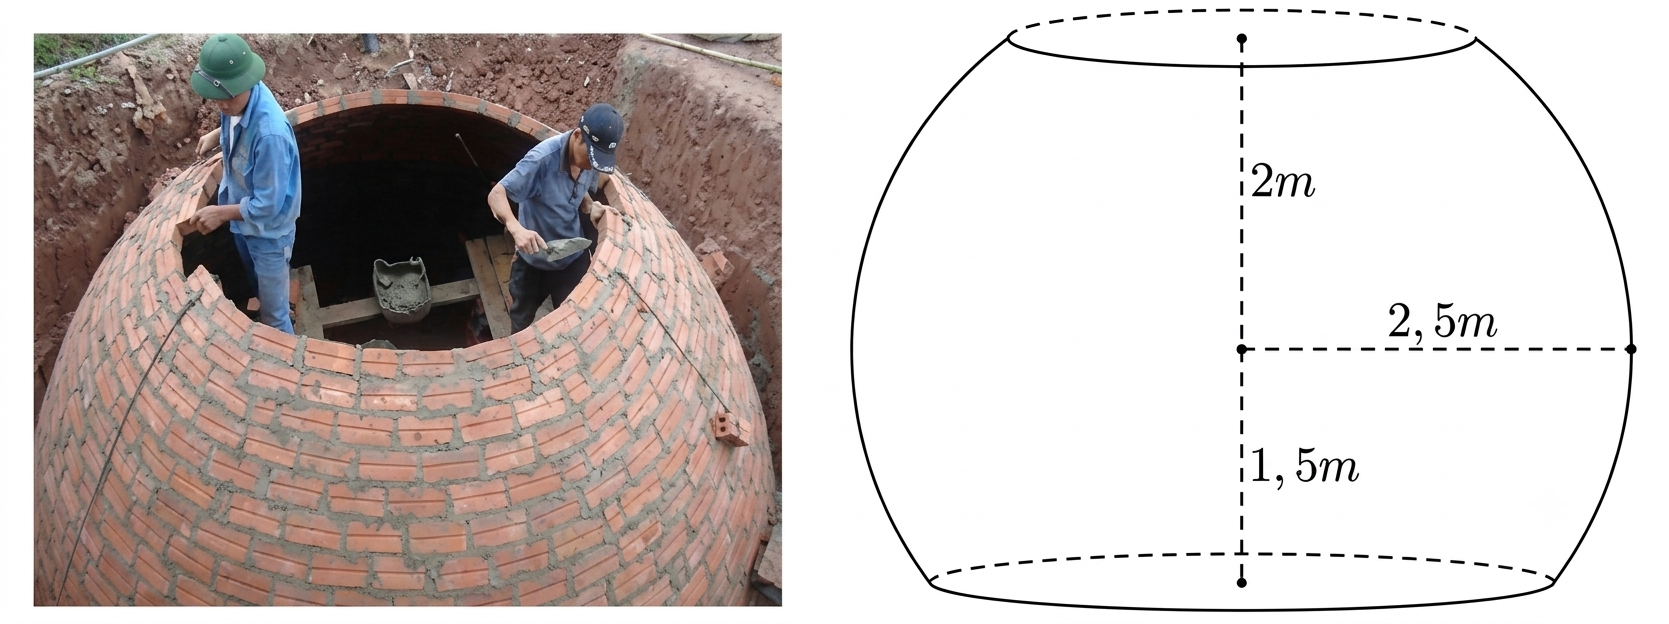
\includegraphics[width=0.6\textwidth]{Cau19.png}
\end{figure}
}

% --- CÂU 20 ---
\questionShortAnswer{0}{20}{Một biển quảng cáo có dạng hình vuông $ABCD$ cạnh $AB = 4\text{ m}$ Trên tấm biển đó có các đường tròn tâm $A$ và đường tròn tâm $B$ cùng bán kính $R = 4\text{ m}$, hai đường tròn cắt nhau như hình vẽ. Chi phí để sơn phần gạch chéo là $150\,000\text{ đồng/m}^2$, chi phí sơn phần màu xám/đen là $100\,000\text{ đồng/m}^2$ và chi phí để sơn phần còn lại là $250\,000\text{ đồng/m}^2$.
\begin{figure}[H]
    \centering
    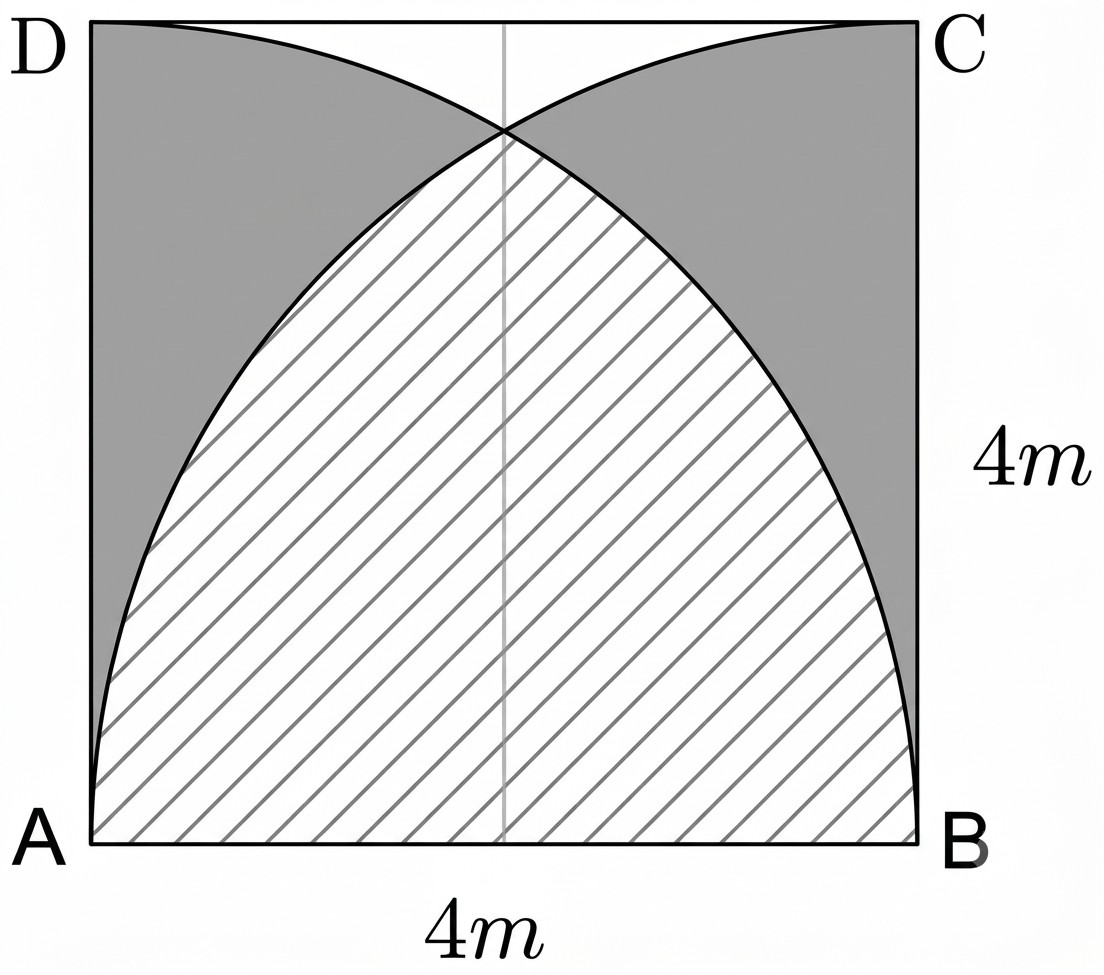
\includegraphics[width=0.3\textwidth]{Cau20.png}
\end{figure}
Hỏi số tiền để sơn biển quảng cáo theo cách trên là bao nhiêu nghìn đồng (kết quả làm tròn đến hàng chục)?}

% --- CÂU 21 ---
\questionShortAnswer{0}{21}{Một người chuyển động trong $3$ giờ với vận tốc $v\text{ (km/h)}$ phụ thuộc thời gian $t\text{ (h)}$ có đồ thị như hình bên. Trong khoảng thời gian $1$ giờ kể từ khi bắt đầu chuyển động, đồ thị đó là một phần của đường parabol có đỉnh $I(2; 9)$ và trục đối xứng song song với trục tung, khoảng thời gian còn lại đồ thị là một đoạn thẳng song song với trục hoành. Tính quãng đường $s$ mà vật di chuyển được trong $3$ giờ đó (kết quả làm tròn đến hàng phần chục).

\begin{center}
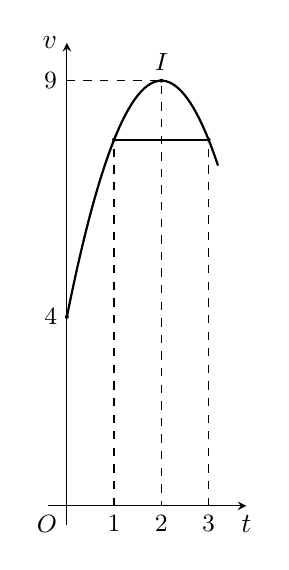
\begin{tikzpicture}[scale=0.6, >=stealth]
    % Trục tọa độ
    \draw[->] (-0.4, 0) -- (3.8, 0) node[below] {$t$};
    \draw[->] (0, -0.4) -- (0, 9.8) node[left] {$v$};
    \node[below left, font=\small] at (0, 0) {$O$};

    % % Parabol nét đứt (toàn phần đỉnh)
    % \draw[dashed, line width=0.6pt, domain=0.8:3.2, samples=60] 
    %     plot (\x, {-1.25*(\x - 2)^2 + 9});

    % Đồ thị vận tốc thực tế (nét liền)
    \draw[thick, domain=0:3.2, samples=50] 
        plot (\x, {-1.25*(\x - 2)^2 + 9});
    \draw[thick] (1, 7.75) -- (3, 7.75);

    % Các đường dóng nét đứt
    \draw[dashed, line width=0.5pt] (0, 9) node[left, font=\small] {$9$} -- (2, 9) node[above, font=\small] {$I$} -- (2, 0) node[below, font=\small] {$2$};
    \draw[dashed, line width=0.5pt] (1, 0) node[below, font=\small] {$1$} -- (1, 7.75);
    \draw[dashed, line width=0.5pt] (3, 0) node[below, font=\small] {$3$} -- (3, 7.75);

    % Tọa độ ban đầu
    \node[left, font=\small] at (0, 4) {$4$};

    % Các điểm mốc
    \fill (0, 4) circle (1.2pt);
    \fill (1, 7.75) circle (1.2pt);
    \fill (3, 7.75) circle (1.2pt);
    \fill (2, 9) circle (1.2pt);
\end{tikzpicture}
\end{center}
}


% --- CÂU 22 ---
\questionShortAnswer{0}{22}{Một vật đang ở nhiệt độ $100^{\circ}\text{C}$ thì được đặt vào môi trường có nhiệt độ $30^{\circ}\text{C}$. Kể từ đó, nhiệt độ của vật giảm dần theo tốc độ $T'(t) = -140e^{-2t}\ (^{\circ}\text{C}/\text{phút})$, trong đó $T(t)$ là nhiệt độ tính theo $^{\circ}\text{C}$ tại thời điểm $t$ phút kể từ khi được đặt vào môi trường. Xác định nhiệt độ của vật ở thời điểm $3$ phút kể từ khi được đặt vào môi trường (kết quả làm tròn đến hàng phần mười của $^{\circ}\text{C}$).}



\end{document}
%1B, 2B, 3C, 4C, 5C, 6C, 7B, 8C, 9A, 10C, 11B, 12A
%13DDSS, 14DSDD, 15DDSS, 16DDSS
%17:1458; 18:1300; 19:56.8; 20:2.2 ;21:21.6; 22: 30.2